This section discusses the methods to identify the presence of hyper giants in today's Internet and to find out the inter dependency between hyper giants and popular websites.To find out the hyper giants in Internet,the hosting infrastructures which are serving popular websites will be observed.DNS resolution on each web site link resolve into single or multiple  IP addresses and corresponding ARecord names.The hosting infrastructures for a web site can be determined by studying the second level domain (SLD) of each ARecord name. The set of IP addresses for a particular SLD shows the degree to which the corresponding SLD infrastructure is network-wise and geographically distributed. The number of bgp prefixes shows the network footprint and the number of ASNs shows how infrastructures are distributed all over the world. For example the highly distributed infrastructures have a lot of prefixes as well as high number of ASNs. Similarly small data centers will be located within a single AS, having a limited number of BGP prefixes, and a large number of IP addresses. Eventually these features are correlated. Hence natural choice for the features to consider are IP addresses, AS Numbers and the BGP prefixes etc. as seen in figure-6. To evaluate the features, HTTP header analysis and DNS resolution will be carried out on Alexa's top 100,000 websites and the website links embedded in these top 100,000 websites. Web object type will be observed from HTTP header information to determine different content types like text/html, image, video, audio etc. and will be examined further to detect the interdependency between hyper giants and the popular websites. DNS resolution will be done on each link to find out corresponding ARecords and IP addresses. These features will be used intensively to evaluate the methods. In the following subsections,the different steps to identify the hyper giants and the inter dependency between hyper giants and popular web sites will be analyzed. 

\begin{figure}[h]
\includegraphics[width=\textwidth,height=10cm]{/home/sakib/soumya/wholeSLD/method-1.png}
\centering
\caption{High level approach Part-1}
\end{figure}

\begin{figure}[h]
\includegraphics[width=\textwidth,height=10cm]{/home/sakib/soumya/wholeSLD/method-2.png}
\centering
\caption{High level approach Part-2}
\end{figure}

\subsection{Identification of hyper giants}
To find out the hyper giants in Internet,the SLD infrastructures which are serving popular websites will be observed. This can be determined by analyzing different features of SLD infrastructures like IP addresses, BGP prefixes, ASN numbers etc. The methods to find out these features will be discussed in the following subsections.
\subsubsection{DNS Resolution}
As can be seen from figure-5, the 100,000  top ranked websites from Alexa will be parsed through scrapy crawler to collect all the links embedded in home pages of these websites.DNS resolution will be done on each link to find out the corresponding ARecord names and IP addresses. The ARecord names which are resolved into final IP addresses will be considered for further analysis.
\begin{figure}[h]
\includegraphics[width=\textwidth,height=10cm]{/home/sakib/soumya/wholeSLD/dnsBmw.png}
\centering
\caption{dig for bmw.com}
\end{figure}
As can be seen from figure-, the website "www.bmw.com" is resolved into several CNAMEs like cn-www.bmw.com.edgesuite.com and a1586.b.akamai.net but a1586.b.akamai.net is  finally resolved into IP addresses 104.121.76.73 and 104.121.76.73. Hence a1586.b.akamai.net will be considered  to identify the SLD infrastructure involve with IP addresses 104.121.76.73 and 104.121.76.73. Mozilla suffix list [https://publicsuffix.org/] will be used to find out SLD infrastructure from the ARecord name.After applying mozilla suffix list on ARecord a1586.b.akamai.net,the SLD infrastructure akamai.net is found. 

\subsubsection{SLD infrastructure analysis}
\begin{figure}[h]
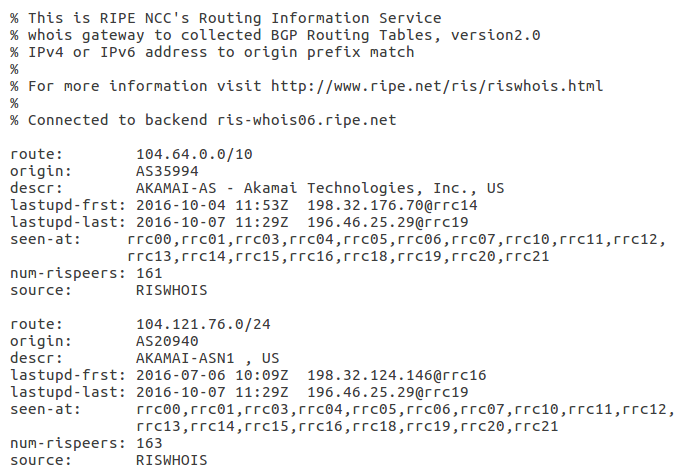
\includegraphics[width=\textwidth,height=10cm]{/home/sakib/soumya/latexNew/whois.png}
\centering
\caption{RIPE RIS bgp prefixes using whois command}
\end{figure}
From the above section, the SLD infrastructure and corresponding IP addresses are determined. To find out BGP prefix routes of a particular IP address, BGP routing information from RIPE RIS [23] will be used. In figure-7, "route" shows the BGP prefixes of a IP address. From the figure this can be seen that the IP address 104.121.76.73 can be routed via two different prefixes 104.64.0.0/10 and 104.121.76.0/24. So both the prefixes for the IP address 104.121.76.73 will be considered for further analysis. This procedure will be carried out for each IP addresses of SLD infrastructure which will be result (SLD,prefixes) mapping.

\subsection{Clustering}
It is found that there are some SLDs which are served by same company. Like akamaiedge.net and akamai.net both are SLD infrastructures used by Akamai company. Similarly google.com, googleusercontent.com, googlehosted.com and googledomains.com all are used by Google. Normally companies used different names when they serve different services to the customer or different name for certain  located customers. This can be seen from the CNAMEs used by amazonaws.us-east-1.elb.amazonaws.com, eu-west-1.elb.amazonaws.com are two examples of naming pattern used by the amazon to provide services to distinct located customers. But here the question arises that these names are pointing to same infrastructure or different. If they are pointing to same infrastructure they should be considered as one, else separately. Hence it is important to identify if these SLDs share same infrastructure or not.This can be identified by using clustering algorithm by analyzing the BGP prefixes they share. 

The clustering algorithm can be divided into two parts.In the first step, the prefixes of a SLD infrastructure will be aggregated into set of parent prefixes and in
the subsequent step, the parent prefixes of the SLD infrastructures will be compared with each other for clustering if they share most of the infrastructures with each other.
\subsubsection{Aggregate Prefixes}
From the above step, SLD infrastructures mapped to corresponding BGP prefixes are collected. But in this mapping, it is observed that some of the BGP prefixes are subset of other BGP prefixes. For example, googledomains.com has the prefix set ’216.239.32.0/19’, ’216.239.32.0/24’, ’216.239.34.0/24’, ’216.239.36.0/24’ and ’216.239.38.0/24’. Here the prefixes ’216.239.32.0/24’, ’216.239.34.0/24’, ’216.239.36.0/24’, ’216.239.38.0/24’ are subnet of prefix ’216.239.32.0/19’.Hence it is ideal way to combine them together. Hence in this aggregation method all the child prefixes will be combined into their parent prefixes for a particular SLD infrastructure. By end of this method the resultant will contain the SLD infrastructure and and prefix set which is incorporate of the parent prefixes, the prefixes which do not have any child in the prefix set. After the above step for googledomains.com, the prefix set will become ’216.239.32.0/19’ as other prefixes are subset of parent prefix 216.239.32.0/19. This procedure will be done for all the SLD infrastructures. Now to cluster two SLD infrastructures, the comparison between their prefix sets will be performed. More details about the similarity procedure will be discussed in the next section.
\subsubsection{Similarity between two prefixes set}
Based on the similarity between prefix sets, the clustering of two SLD infrastructures will be determined. While comparing between two SLD infrastructures, if any of the SLD infrastructure contain child prefix of other, then the child prefix will be replaced with parent prefix. This will make two prefix set with only parents. Now compare the two sets of prefixes to find out whether they are sharing same infrastructure or not. For comparing two SLD infrastructures, the similarity equation is defined as follows,

\begin{equation}
similarity(s1, s2)= \frac{|s1 \cap s2|}{|s2|}
\end{equation}

where s1,s2 are the bgp prefix sets.

If the similarity between two prefix sets are greater than equal to 70\% then both the SLD infrastructures will be clustered together. Here the assumption is taken as, if s2’s 70\% prefixes are present in the common infrastructure between s1 and s2 set,then it shows
that s2 sharing most of the infrastructure of s1. Hence both infrastructures can be clubbed together. This procedure will be done for all the SLDs. If two SLDs are matched ,then the child SLD infrastructure will be removed from comparison with other SLDs and it will be mapped to the SLD with which it matched.For example ’googleusercontent.com’ matched with ’google.com’ with similarity 100\%. Once this is matched googleusercontent.com and 
google.com clubbed together and ’googleusercontent.com’ will not be available for any further similarity matching with any other SLD infrastructures. 70\% of similarity is chosen after extensively testing between bgp prefixes.
\subsubsection{Evolution of hyper giants}
Now after the clustering procedure, clustered SLD infrastructures will be determined
under each of which multiple number of SLD infrastructures are collected based on similarity comparison between two SLD infrastructures. To find out hyper giants presence, the features of each clustered SLD infrastructures will be analyzed.The features include number of links, number of IP addresses, number of BGP prefixes, number of AS numbers. To find out each of these features for a  clustered SLD infrastructure, corresponding SLD infrastructures clubbed  under same clustered SLD infrastructure will be considered.Hence total number of links for a clustered SLD infrastructure will be the sum of all the links served by all SLD infrastructures clubbed under same clustered SLD infrastructure.Similar procedure will be taken to find out other features.The features will be analyzed further to find out the hyper giants.
\subsection{Web objects delivered from hyper giants to popular web sites}
To find out different web objects delivered from hyper giants to popular web sites, HTTP header information for a SLD infrastructure will be analyzed.From header information,the content type of each object can be observed.Hence to find out different types of web objects delivered through hyper giants, web objects served through each clustered SLD infrastructures will be determined first.This can be done by summing of all the web objects served by all SLD infrastructures clubbed under same clustered SLD infrastructure. 
\subsection{Conclusion}
This section discussed about the methods to identify the presence of hyper giants in today's Internet and to find out the inter dependency between hyper giants and popular websites. To achieve both the methods ,natural choice for the features to consider are IP addresses, AS numbers and the BGP prefixes.The section provided the procedures to find out each of the features for SLD infrastructures. At the end, a mechanism to find out how far different types of web objects delivered from hyper giants to popular web sites is discussed.